
\section{Design and implementation}
Our main goal when designing \oursys was to preserve a standard \sockets API, while providing seamless zero-copy I/O support. A secondary goal is to eliminate costly system calls from the data path. 

We can classify the existing zero copy techniques into four categories:
\begin{enumerate}
    \item Dynamic remapping (e.g., tcp\_mmap, MSG\_ZEROCOPY\cite{desendmsg}, mikelangelo-project\cite{mikelangelo}).
    \item Kernel Bypass (e.g., DPDK, Netmap\cite{rizzo2012netmap}).
    \item Special/Limited use-case (splice, sendfile).
    \item Shared buffers (e.g, INSTANCE \cite{instance}).
\end{enumerate}
Out of the four categories only \#1 and \#4 allow for a generic use of standard \sockets API. Due to mainly security concerns examples that fit into category \#4 are the rarest.
While there are many examples to solutions that fall into category \#1 \cite{mikelangelo-empty,desendmsg}, but they usually discover that modifying virtual memory on the fly is computationally expensive. 

For these reasons we have decided that we should look into a Shared buffer solution. Our inspiration for a correct shared buffer solution comes from a similar problem in IOMMU security. DAMN \cite{markuze2018damn}, creates a memory allocator based on a pool of perpetually DMA mapped buffers, which are used for I/O by the Linux Network stack and device drivers. This solution effectively creates a \emph{secure} shared memory solution between the Server and the NIC.

We propose \oursys, a Memory Allocator for I/O, for the  exclusive use of the network stack. The \oursys allocator uses a pool of dedicated compound memory pages(i.e., \_\_GFP\_COMP). We adopt the allocation mechanics proposed in DAMN\cite{markuze2018damn}. I.e., the allocator is based on two known mechanisms; a page\_frag mechanism \cite{pagefrag} over \size buffers, these buffers in turn are allotted by a magazine allocator \cite{bonwick2001magazines}. This allocation scheme allows for efficient allocation of variable size buffers in the kernel. Variable size allocations is needed to support variable sizes of MTU and HW offloads (e.g., HW GRO). 
To facilitate zero copy, these pages are mapped \emph{once} to the virtual memory address space of the privileged user-space process. In order to use \oursys, the user-space program, has to mmap the \oursys buffer and then allocate a virtual region for its own use (i.e., zero-copy send), the size of the allocated region should be a multiple of \size. A second way the user-space process can get \oursys buffers, is by performing zero-copy receive. The user-space process can return memory to the kernel via a exception-less mechanism described in Sec. \ref{sec:bifurcated}.
The \oursys buffers are depicted in Fig. \ref{fig:our_sys} as dashed boxes.
%That process is now able of perform zero-copy I/O.
\subsection{Bifurcated I/O}\label{sec:bifurcated}
A second issue that impacts user space I/O performance, is the direct and indirect cost of system calls\cite{flexsc}.
To avoid the costly operation of invoking a costly system calls we offload the I/O operation to a dedicated kernel thread (Fig. \ref{fig:our_sys} \textbf{(3)}) which will perform the I/O operation using kernel sockets \cite{ktcp}. For example a \texttt{send\_msg} system call is replaced with an I/O descriptor (i.e., \texttt{struct msghdr} and \texttt{int flags}) written to a shared memory ring buffer (Fig. \ref{fig:our_sys} \textbf{(2)}). This form of splitting the responsibility for performing I/O preservers the existing socket API, facilitates exception-less system calls, and allows for better parallel programming. Bifurcated I/O enables the separation of the application computations and the TCP computations to different CPU cores. Both zero-copy and standard send are supported, in standard mode the sent buffer is copied to a new \oursys buffer before send. Supporting standard mode of send is benefitialk for applications performing small I/O e.g., 64B sends (we evaluate the costs in Sec .\ref{sec:eval_bif}).
%RX: just poll the descriptor ring or sleep with sys call.
%TX: continuous poll. NAPI like execution, with amortized sys call, when not polling.

\begin{figure}[t]
    \centering
    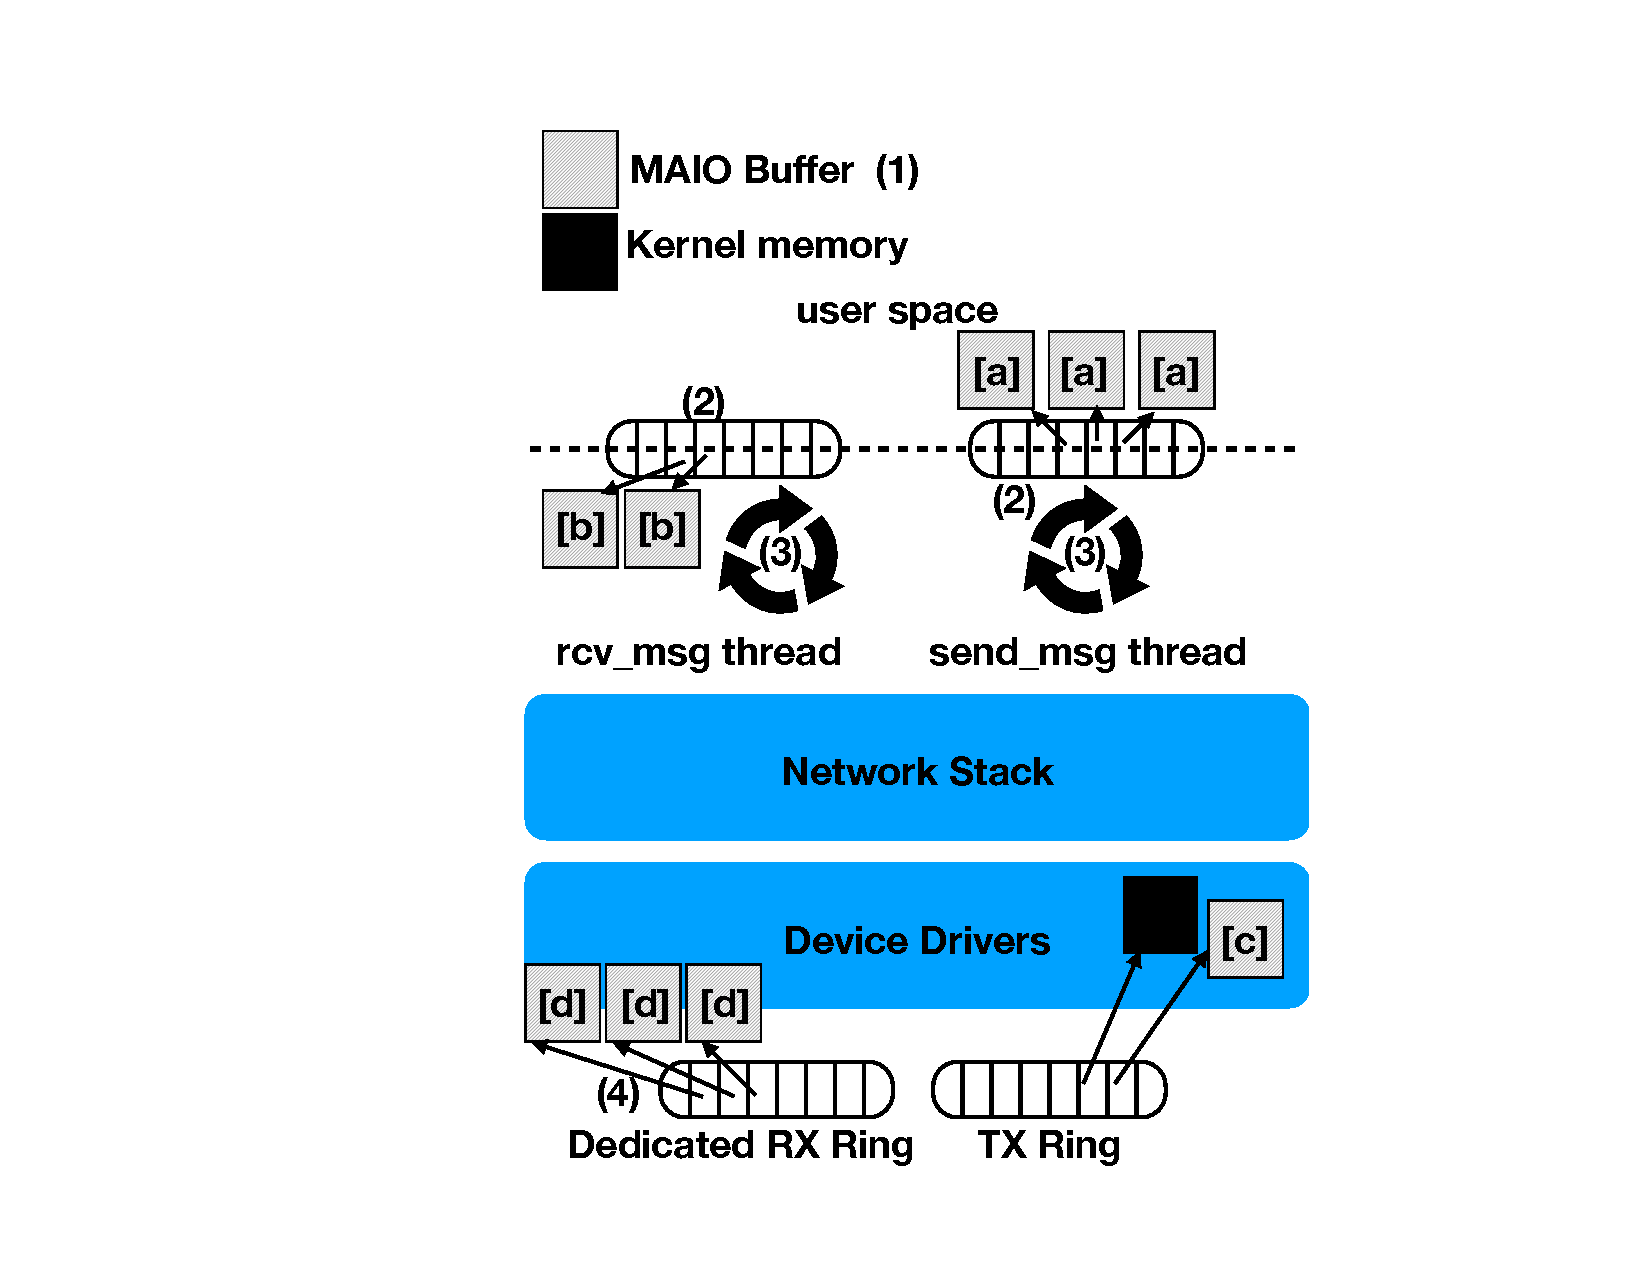
\includegraphics[width=0.8\columnwidth]{ktcp_z.pdf}
    \caption{1. \oursys shared memory buffers 2. shared io rings for exception-less system calls 3. A kernel thread executing I/O operations 4. A dedicated RX ring.
    [a] zero-copy send\_msg [b] zero-copy recvmsg [c] \oursys buffer in driver TX ring [d] \oursys buffers used by the device driver for RX}
    \label{fig:our_sys}
\end{figure} 

\subsection{Security}
Such a solution initially razes concerns about the security and stability of the system, as the process now \emph{seemingly} has access to sensitive kernel memory. 

\noindent\textbf{Driver Support.} We can allocate dedicated NIC RX rings for \oursys users. HW support\cite{flow_direct} can direct a single 5 tuple (or a defined group of 5 tuples). Limiting the shared buffers \emph{only} to this users data. The implementation of a driver support, is out of the scope of this work. 

\noindent\textbf{Kernel Security.} \oursys is integrated in such a way that the shared pages are only ever used by the Kernel to hold the I/O \emph{data} buffers and \emph{not} the meta data or any other kernel need. Namely, the process can only ever see the information it has written or data bound to user-space. In addition to the data, the process is privy to the transport headers as well; we assume the NIC supports Header/Data splitting\cite{hds} which can place the headers onto non-shared buffers.

\noindent\textbf{User Security.} By sharing all potential RX buffers \oursys exposes all traffic to a single observer.
Without driver support this limits the usefulness of \oursys to those cases when the user is trusted (e.g., sudo). 

\subsection{Shared buffer concerns.}
\noindent\textbf{Kernel Starvation.} The user process may hoard \oursys buffers without releasing them to the kernel.
In this case the driver will revert to standard  memory allocation, and will render the application unable to receive , while other process and kernel functionality will remain unchanged.


\noindent\textbf{Pinned pages.} In early solutions proposed for zero-copy by shared static buffer, were considered dangerous because these shared pages can be exhausted and cannot be swapped out \cite{song2012performance,yamagiwa2005active}. We contend that this is not a real concern for modern systems as systems with hundreds of GB are the norm. Key/Value applications (e.g., memcached, redis) expect their memory to be persistent in memory. Additionally HPC applications, many\cite{top500} of which use RDMA, \texttt{register} (i.e., pin to memory) large memory regions that are then used for I/O.

\subsection{zero copy support for kernel sockets}
We expand the existing Linux TCP API with a \texttt{tcp\_read\_sock\_zcopy} for \texttt{RX} and add a new msg flag \texttt{SOCK\_KERN\_ZEROCOPY} for \texttt{tcp\_sendmsg\_locked} in \texttt{TX}. We base our new function \texttt{tcp\_read\_sock\_zcopy} on existing infrastructure i.e., \texttt{tcp\_read\_sock}. It is used by \texttt{tcp\_splice\_read} to collect buffers from a socket without copying. For \texttt{TX}, zero copy infrastructure already exists in the form of MSG\_ZEROCOPY\cite{desendmsg}. When kernel memory is used for I/O, enabling zero copy is trivial when compared to zero copy from user space. The pages are already pinned in memory and there is not need for a notification on \texttt{TX} completion. The pages are reference counted, and can be freed by the device driver completion handler.


For TX instead of modifying the behavior of \texttt{tcp\_sendmsg\_locked}, its also possible to use \texttt{do\_tcp\_sendpages}, which is used in splice. Ironically, \texttt{do\_tcp\_sendpages} accepts only one page fragment (i.e., \texttt{struct page}, size and offset) per invocation and does not work with a scatter-gather list, like \texttt{tcp\_sendmsg\_locked}.

%Related to FlexSC \cite{flexsc}, \\TODO:\\
%1. ~/memory\_trace/poller/\\
%2. rerun context switch tests?